\documentclass[12pt]{matmex-diploma}
\usepackage[numbers]{natbib}
\usepackage{hyperref}
\usepackage{amsmath}
\usepackage{amssymb}
\usepackage{amsthm}
\usepackage{mathtools}
\usepackage{tikz}
\usepackage{tikz-cd}
\usepackage{subdepth}
\usepackage{indentfirst}
\usetikzlibrary{calc}
\usetikzlibrary{patterns}
\usetikzlibrary{decorations.pathreplacing}
\usepackage[most]{tcolorbox}
\usepackage{enumitem}
\usepackage{cancel}

\usepackage{fontspec}
\setmainfont{Times New Roman}
\defaultfontfeatures{Mapping=tex-text}
\newfontfamily\cyrillicfont{Times New Roman} 

\makeatletter
\newcounter{aaa}
\tikzset{
  apply/.style args={#1 except on segments #2}{postaction={
      /utils/exec={
        \@for\mattempa:=#2\do{\csdef{aaa@\mattempa}{}}
        \setcounter{aaa}{0}
      },
      decorate,decoration={show path construction,
        moveto code={},
        lineto code={
          \stepcounter{aaa}
          \ifcsdef{aaa@\theaaa}{}{
            \path[#1] (\tikzinputsegmentfirst) -- (\tikzinputsegmentlast);
          }
        },
        curveto code={
          \stepcounter{aaa}
          \ifcsdef{aaa@\theaaa}{}{
            \path [#1] (\tikzinputsegmentfirst) .. controls
            (\tikzinputsegmentsupporta) and (\tikzinputsegmentsupportb)
            ..(\tikzinputsegmentlast);
          }
        },
        closepath code={
          \stepcounter{aaa}
          \ifcsdef{aaa@\theaaa}{}{
            \path [#1] (\tikzinputsegmentfirst) -- (\tikzinputsegmentlast);
          }
        },
      },
    },
  },
}
\makeatother

\makeatletter
\newcommand*{\shifttext}[2]{%
  \settowidth{\@tempdima}{#2}%
  \makebox[\@tempdima]{\hspace*{#1}#2}%
}
\makeatother



\filltitle{ru}{
    chair              = {\hspace{8em} 01.04.01 Математика \tiny ---  царица \xcancel{полей} ${}^{\text{\textit{коммутативных колец}}}$},
    title              = {Линейные алгебраические группы,\\ сходные с параболическими},
    % Здесь указывается тип работы. Возможные значения:
    %   coursework - Курсовая работа
    %   diploma - Диплом специалиста
    %   master - Диплом магистра
    %   bachelor - Диплом бакалавра
    type               = {master},
    position           = {студента},
%    group              = 123,
    author             = {Буряков~Михаил~Александрович},
    supervisorPosition = {д.\,ф.-м.\,н., профессор},
    supervisor         = {Вавилов~Н.\,А.},
    reviewerPosition   = {к.\,ф.-м.\,н., доцент},
    reviewer           = {Певзнер И.\,М.},
    %chairHeadPosition  = {д.\,ф.-м.\,н., профессор},
    %chairHead          = {Хунта К.\,Х.},
    university         = {Санкт-Петербургский Государственный Университет},
    faculty            = {Математико-механический факультет},
%    city               = {Санкт-Петербург},
%    year               = {2013}
}

\newtheoremstyle{mystyle}%       % Name
  {}%                            % Space above
  {}%                            % Space below
  {\itshape}%                    % Body font
  {}%                            % Indent amount
  {\upshape\bfseries}%           % Theorem head font
  {. }%                          % Punctuation after theorem head
  { }%                           % Space after theorem head, ' ', or \newline
  {}%                            % Theorem head spec (can be left empty, meaning `normal')
  
\newtheoremstyle{mystyleni}%       % Name
  {}%                            % Space above
  {}%                            % Space below
  {}%                            % Body font
  {}%                            % Indent amount
  {\upshape\bfseries}%           % Theorem head font
  {. }%                          % Punctuation after theorem head
  { }%                           % Space after theorem head, ' ', or \newline
  {}%                            % Theorem head spec (can be left empty, meaning `normal')
    
  
\newlength{\normalparindent}
\AtBeginDocument{\setlength{\normalparindent}{\parindent}}
\tcbset{before upper={\setlength{\parindent}{\normalparindent}}}
  
  
\makeatletter
\newcommand{\slunlhd}{%
  \mathrel{\mathpalette\sl@unlhd\relax}%
}

\newcommand{\sl@unlhd}[2]{%
  \sbox\z@{$#1\lhd$}%
  \sbox\tw@{$#1\leqslant$}%
  \dimen@=\ht\tw@
  \advance\dimen@-\ht\z@
  \ifx#1\displaystyle
    \advance\dimen@ .2pt
  \else
    \ifx#1\textstyle
      \advance\dimen@ .2pt
    \fi
  \fi
  \ooalign{\raisebox{\dimen@}{$\m@th#1\lhd$}\cr$\m@th#1\leqslant$\cr}%
}
\makeatother

\theoremstyle{mystyleni}
\newtheorem{hyp}{Свойство}

\theoremstyle{mystyle}
\newtheorem{thm}{Теорема}
\newtheorem{lm}{Лемма}
\newtheorem{rem}{Замечание}
\newtheorem{example}{Пример}
\newtheorem{definition}{Определение}

\newenvironment{framed}
    {
\vspace{1.5ex}
\begin{tcolorbox}[colback=white, grow to left by=1.2em, grow to right by=1.2em, enhanced]
    }
    {
\end{tcolorbox}
    }

\newcommand\refb[1]{\textbf{\ref{#1}}}

\newcommand{\Z}{\mathbb{Z}}
\newcommand{\N}{\mathbb{N}}
\renewcommand{\C}{\mathbb{C}}
\renewcommand{\le}{\leqslant}
\renewcommand{\ge}{\geqslant}
\renewcommand{\trianglelefteq}{\slunlhd}

\def\lacts{\curvearrowright}
\def\racts{\curvearrowleft}

\newcommand\bigzero[2]{\raisebox{#2ex-2ex}[0pt][0pt]{\shifttext{#2em}{\text{\Huge{#1}}}}}

\linespread{1.25}
\fontdimen2\font=0.35em

\begin{document}

\maketitle
\tableofcontents


\newcommand\placeholder{\textcolor{red}{\textbf{\\\#\\\#\\\#}}}

\newpage
\section{Введение}

Теория линейных алгебраических групп над коммутативными кольцами является обобщением теории линейных алгебраических групп над полями и изучается с 60-х годов XX века.
Структурная теория и нормальное строение групп Шевалле и редуктивных групп достаточно хорошо изучены. В работе А.~В.~Степанова \citep{Stepanov1991} вводится понятие "стандартного" расположения подгрупп, нормализуемых некоторой фиксированной подгруппой.

Доказательства стандартности расположения подгрупп в группах Шевалле и редуктивных группах, нормализуемых элементарной подгруппой, приводятся для различных случаев в работах И.~Абе \citep{Abe1989}, Л.~Н.~Васерштейна \citep{Vaserstein1988}, И.~З.~Голубчика \citep{Golubchik1975}, Р.~Хазрата, В.~А.~Петрова и Н.~А.~Вавилова \citep{Hazrat2010}, А.~К.~Ставровой и А.~В.~Степанова \citep{Stavrova2018} и др. Более явные доказательства структурных теорем для групп Шевалле над коммутативными кольцами приводятся в статье Н.~А.~Вавилова, М.~Р.~Гавриловича, С.~И.~Николенко \citep{Vavilov2006}, а в статье Р.~Пройссера \citep{Preusser2018} предлагается новая схема доказательства "стандартного" расположения подгрупп, нормализуемых элементарной, в классических группах.


Интерес также представляют и нередуктивные группы.
Например, нормальное строение параболических подгрупп в группах Шевалле изучается в работах \citep{Azad1990}, \citep{Roehrle1998}, \citep{Stavrova2009}. В частности, в работе А.~К.~Ставровой \citep{Stavrova2009} приводится описание подгрупп максимальной параболической группы, нормализуемых элементарной подгруппой Леви.
Методы исследования, используемые в работе \citep{Stavrova2009}, могут быть применены не только к параболическим подгруппам групп Шевалле и редуктивных групп, но и к более широкому классу нередуктивных групп. 

Целью данной работы является описание нормального строения некоторого класса нередуктивных групп, которые строятся на основе линейного представления редуктивной группы, и по своим свойствам сходны с параболическими подгруппами групп Шевалле.
Исследуемая задача имеет весьма высокую научную значимость, о чём свидетельствуют многочисленные публикации с доказательствами различных теорем о нормальном строении линейных групп над коммутативными кольцами.

Работа устроена следующим образом: во втором разделе изложены некоторые предпосылки к формулировке задачи, третий и четвёртый разделы содержат базовые определения и факты, необходимые для формулировки основного результата. В пятом разделе вводится определение параболически-сходных групп с абелевым унипотентным радикалом. Следующие два раздела содержат формулировку и доказательство основного результата работы о нормальном строении параболически-сходных групп с абелевым унипотентным радикалом. В восьмом разделе обсуждается существенное условие, возникающее в доказательстве основного результата, и влияние этого условия на расположение подгрупп, нормализуемых элементарной.
В последнем разделе работы даются предпосылки для возможного обобщения результатов о нормальном строении параболически-сходных групп на параболически-сходные группы с неабелавым унипотентным радикалом.


\section{Постановка задачи}

Одной из предпосылок к постановке задачи послужила следующая проблема. 
Рассмотрим \emph{ортогональную группу} $\mathrm{O}(B)$ --- группу автоморфизмов $R$-модуля $V$, сохраняющих билинейную форму $B$:
$$ \mathrm{O}(B) = \{ g \in \mathrm{GL}(V) \,|\, B(gx,gy) = B(x,y) \; \forall x,y \in V \} $$

Во многих работах, изучающих структурную теорию этой группы, предполагается невырожденность формы $B$.
Но даже в тех работах, где требования невырожденности нет (например, в работе В.~А.~Петрова \cite{Petrov2005}), элементарная подгруппа определяется через трансвекции Эйхлера-Зигеля-Диксона:
$$ T_{uv}(\xi) : w \mapsto w + u (B(v,w) + \xi B(u,w)) + v B(u,w) \;, $$
где $ B(u,u) = B(u,v) = 0$.

Очевидно, если билинейная форма вырожденная (в частности, если она имеет вид $B \oplus 0$), то элементарная группа, определённая таким образом, существенно меньше всей группы.

Такого вида ортогональные группы уже не будут редуктивными над тем кольцом, над которым форма вырождена. Их структура достаточно близка к структуре параболческих подгрупп в группах Шевалле, хотя они в общем случае могут не вкладываются в группы Шевалле в качестве параболических подгрупп. Это сходство послужило отправной точкой для изучения более общего класса нередуктивных групп, включающего оба случая: параболические подгруппы групп Шевалле и вырожденные ортогональные группы. Структурной теории предложенного обобщения --- \emph{группам, сходным с параболическими} --- и посвящена данная работа.

Как известно из работы \citep{Azad1990}, на унипотентном радикале параболической подгруппы можно ввести структуру модуля, так что на некотором его фактормодуле действует подгруппа Леви. Введение понятия \emph{групп, сходных с параболическими} имеет целью "обратить" данную конструкцию, то есть явным образом конструировать группу из некоторого заданного представления.
%Таким образом сконструированные группы будем называть \emph{группами, сходными с параболическими}.

\pagebreak
\section{Определения}

\begin{comment}
Следующие три определения широко известны и приведены, например, в работах \cite{Conrad11reductivegroup}, \#, \#.
\begin{definition} 
Редуктивной $R$-группой называется линейная алгебраическая $R$-группа, не содержащая нетривиальных связных нормальных унипотентных линейных алгебраических $R$-подгрупп.
\end{definition}

\begin{definition}
Полупростой $R$-группой называется линейная алгебраическая $R$-группа, не содержащая нетривиальных связных нормальных разрешимых линейных алгебраических $R$-подгрупп.
\end{definition}

\begin{definition}
Простой $R$-группой называется линейная алгебраическая $R$-группа, не содержащая нетривиальных связных нормальных линейных алгебраических $R$-подгрупп.
\end{definition}
\end{comment}

В настоящей работе используются следующие обозначения из теории групп.\linebreak
Пусть $G$ --- произвольная абстрактная группа. Коммутатор элементов $x$ и $y$ из $G$ будем обозначать как $[x,y]=x y x^{-1} y^{-1}$.
Выражение $x y x^{-1}$ кратко будем записывать ${}^x y$.

Если $X \subseteq G$ --- подмножество группы $G$, тогда под $\left<X\right>$ будем понимать подгруппу, порожденную $X$.
Запись $H\le G$ означает, что $H$ --- подгруппа $G$.
Если $H$ --- нормальная подгруппа в $G$, то это записывается как $H \trianglelefteq G$. В случае, если $H \le G$, запись $\left<X\right>^H$ означает наименьшую подгруппу в $G$, которая содержит $X$ и которая нормализуется $H$.
Полупрямое произведение двух групп $G$ и $F$ обозначается через $G\rightthreetimes F$, где $F$ --- нормальный сомножитель.
Запись $[F,H]$ для двух подгрупп $F,H \le G$ обозначает их взаимный коммутант:
$$ [F,H] = \{[f,g] \, | \, f\in F, g \in G  \} .$$


Известно, что всякой приведённой неприводимой системе корней $\Phi$ единственным образом соответствует односвязная аффинная групповая схема $G(\Phi,-)$ над $\Z$, называемая групповой схемой Шевалле-Демазюра (\cite{Plotkin1998}, \cite{Steinberg2016}, \cite{Chevalley1960-1961}).
Под представлением алгебраической группы $G$ над кольцом $k$ будем понимать гомоморфизм групповых схем $G \to \mathrm{GL}_n(k)$. Это означает, что представление над базовым кольцом индуцирует с помощью расширения скаляров представление над расширенным кольцом.

Представление (над некоторым полем $k$) называется неприводимым (в терминологии \cite{Milne2017} простым), если оно не содержит нетривиальных подпредставлений.
Неприводимые представления редуктивных групповых схем над полем представляют собой модули старшего веса (\cite{Jantzen1987}, следствие 2.7).




Пусть $G_\Z$ --- связная расщепимая редуктивная групповая схема с системой корней $\Phi = \Phi_1 + \dots + \Phi_n$, где $\Phi_i$ --- приведённые неприводимые системы корней, $n \ge 1$.
\linebreak
Далее пусть $\pi:G_\Z \to GL(U_\Z)$ --- представление $G_\Z$ над $\Z$, становящееся неприводимым над алгебраически замкнутым полем характеристики $0$. Тогда $U_\Z$ --- конечномерный свободный модуль старшего веса (\cite{Conrad11reductivegroup}). Будем в дальнейшем предполагать, что его ранг
\begin{equation*}
\mathrm{rk} \; U_\Z \ge 2 \;.
\end{equation*}
Тогда если $R$ --- произвольное коммутативное кольцо, то $\pi$ индуцирует действие группы $G=G_\Z(R)$ на модуле $U = U_Z \otimes R$,  которое будем обозначать следующим образом:
$$ \pi_R(g) : u \mapsto {}^g u \; . $$

Так как $\pi$ является морфизмом схем, то $U$, как и $U_\Z$, будет являться свободным модулем, и в случае выбора максимального тора $T$ является (\citep{Borel1970}) прямой суммой весовых подпространств
$$U=\bigoplus_{\sigma \in \Sigma \subset X(T)} {U \cap U_\sigma} ,$$
где
\begin{equation*}
\begin{split}
& U_\sigma = \{x \in U_\C \; | \; ^h x = \sigma(h) x \; \forall h \in T \},\\
& \Sigma = \{\sigma \in X(T) \; | \; U_\sigma \ne \varnothing\} \text{ --- множество весов представления,}\\
& X(T) \text{ --- группа рациональных характеров тора.}
\end{split}
\end{equation*}

\section{Корневые элементы и их действие}

Известно (\citep{Milne2017}, раздел 19.11), что для каждого корня $\alpha \in \Phi_i$ в $G$ задана \emph{корневая подгруппа} $X_\alpha(R)$, изоморфная аддитивной группе кольца и состоящая из \emph{корневых элементов} $x_\alpha(\xi)$,~$\xi \in R$. Подгруппу в $G$, порождаемую всеми корневыми элементами $x_\alpha(\xi)$, где $\alpha \in \Phi$,~$\xi \in R$, будем обозначать $E = E(\Phi,R)$. 
Подгруппу в $G$, порождаемую всеми корневыми элементами $x_\alpha(\xi)$, где $\alpha \in \Phi^+$ --- положительные корни, $\xi \in R$, будем обозначать $EB = EB(\Phi,R)$. и называть \emph{элементарной борелевской  подгруппой}.
Для каждого идеала $I \trianglelefteq R$ также будем обозначать
$X_\alpha(I) := \left<x_\alpha(\xi) \,|\, \xi \in I\right>$ и $E(\Phi,I) := \left<x_\alpha(\xi) \,|\, \alpha \in \Phi \, \xi \in I\right>$. Нормальное замыкание $E(\Phi,I)$ в $E(\Phi,R)$ будем называть \emph{относительной элементарной подгруппой} и обозначать $E(\Phi,R,I):=E(\Phi,I)^{E(\Phi,R)}$.

Перечислим основные свойства корневых элементов $x_\alpha(\xi)$:
\begin{itemize}[label={\LARGE\raisebox{-0.4ex}{\textbullet}\;},leftmargin=2\parindent]
\item
Для экстремальных весов (в частности, для старшего веса $\widetilde\sigma$), весовые пространства $U_\sigma$ одномерны.
\item
Операторы, соответствующие в конечномерном представлении $\pi_R$ корневым элементам, унипотентны:
$$\exists n : (\pi(x_\alpha(\xi))-1)^n = 1$$
Для базисных представлений (микровесовые представления, представления на коротких корнях и присоединённые представления групп с системами корней с простыми связями, \cite{Plotkin1998}) это верно уже при $n=3$. Для микровесовых представлений это верно уже при $n=2$.
\item
Корневые элементы аддитивны по параметру:
$$x_\alpha(\xi) \; x_\alpha(\theta)  = x_\alpha(\xi+\theta)$$
$$x_\alpha(\xi)^n = x_\alpha(n \, \xi) \; \forall n \in \Z$$
\end{itemize}

На модуле $U$ корневыем элементам $x_\alpha(\xi)$ соответствуют операторы $\pi(x_\alpha(\xi))$. Поэтому, eсли в базовом кольце числа $2 \ldots n-1$ обратимы, то определён логарифм этих операторов, который является от них полиномиальной функцией:
$$ \varepsilon_\alpha(\xi) \coloneqq \mathrm{ln} \, \pi(x_\alpha(\xi)) = \sum_{i=0}^{n-1} {\pi(x_\alpha(\xi))^i k_i} $$
При этом имеется изоморфизм (над базовым кольцом) между корневыми подгруппами $X_\alpha=\left<x_\alpha(\xi)\right>$ и циклическими группами, порождёнными $\varepsilon_\alpha(\xi)$.

Можно видеть, что умножение параметра на целое число эквивалентно умножению на число самого оператора $\varepsilon_\alpha(\xi)$:
$$ \varepsilon_\alpha(n \, \xi) = \mathrm{ln} \, \pi(x_\alpha(n \, \xi)) = \mathrm{ln} \, \pi(x_\alpha(\xi))^n = n \; \mathrm{ln} \, \pi(x_\alpha(\xi)) = n \; \varepsilon_\alpha(\xi) \; \forall n \in \Z
$$

Так как изоморфизм  между циклическими группами $\left<x_\alpha(\xi)\right> \le G$ и $\left<\varepsilon_\alpha(\xi)\right> \le \mathrm{GL}(U)$ определён над базовым кольцом, то аналогичным образом выглядит умножение параметра на произвольные константы:
$$
\varepsilon_\alpha(\eta \, \xi) = \eta \; \varepsilon_\alpha(\xi) \; \forall \eta \in R
$$

\begin{lm}
Оператор $\varepsilon_\alpha(\xi)$ переводит элементы из подпространства $U_\sigma$ в подпространство $U_{\sigma+\alpha}$.
\end{lm}
\begin{proof}
\begin{multline*}
^h(\varepsilon_\alpha(\xi) \, u) =
^h\left(\sum_i \, {^{\pi(x_\alpha(\xi))^i}u \, k_i}\right) = 
\sum_i \, {^{h \pi(x_\alpha(\xi))^i}u \, k_i} = \\ =
\sum_i \, {^{(^h \pi(x_\alpha(\xi)))^i h}u \, k_i} = 
\sum_i \, {^{(\pi(x_\alpha(\alpha(h)\cdot\xi)))^i} \left(^h u\right) \, k_i} =\\=
\sum_i \, {^{(\pi(x_\alpha(\alpha(h)\cdot\xi)))^i} u \cdot \sigma(h) \, k_i} =
\varepsilon_\alpha(\alpha(h)\cdot\xi) \, u \cdot \sigma(h) = \\ =
\varepsilon_\alpha(\xi) \, u \cdot \alpha(h)\sigma(h)
\end{multline*}
\end{proof}

Следующее требование, которые мы в дальнейшем будем предполагать выполненным, относится одновременно к модулю $U$ и кольцу $R$. Для базисных представлений без нулевого веса оно выполнено всегда независимо от кольца $R$, но для более сложных случаев оно может означать обратимость в $R$ некоторых целых чисел.

\vspace{1ex}
\begin{framed}
\begin{hyp}\label{returnfromhighest}
Если $u$ --- некоторый вектор из $U_\sigma$, и $V={}^{EB}\left<u\right>$ --- минимальный \linebreak
$EB$-инвариантный подмодуль, содержащий $u$, то $u \in {}^E\left<V \cap U_{\widetilde\sigma}\right>$, или, что то же самое, ${}^E\left<V \cap U_{\widetilde\sigma}\right> = {}^E \left<u\right>$.

Иными словами, если $u$ --- некоторый вектор из $U_\sigma$, то его образы в пространстве $U_{\widetilde\sigma}$ старшего веса под действием операторов 
$\left(\prod_{\alpha_i}\varepsilon_{\alpha_i}(1)\right)$, где $\alpha_i$ пробегает по всем цепочкам положительных корней, так что $\sum_i \alpha_i = \widetilde\sigma - \sigma$, не содержатся ни в каком $E$-инвариантном модуле, в котором бы не содержался $u$. Иными словами, все эти образы в совокупности порождают (как $E$-инвариантный подмодуль) тот же самый подмодуль, который порождается (как $E$-инвариантный подмодуль) исходным вектором $u$.
\end{hyp}
\end{framed}

Следующие утверждения вытекают из данного свойства:
\begin{lm} \label{extremalweightisomorphism}
Пусть $\sigma$ и $\sigma+n\alpha$ --- экстремальные корни и при этом $u\in U_\sigma$.\linebreak
Тогда если~$(\varepsilon_\alpha(1)^n \, u) $~содержится в некотором $E$-инвариантном подмодуле $V$,\linebreak
то обязательно $u \in V$.
\end{lm}
\begin{proof}
Если $\sigma+n\alpha = \widetilde\sigma$ --- максимальный корень, то утверждение является частным случаем свойства \refb{returnfromhighest}. В остальных случаях $\sigma+n\alpha$ переводится в $\widetilde\sigma$ некоторым элементом группы Вейля.
\end{proof}

\begin{lm}\label{weightprojections}
Если $V$ --- инвариантный подмодуль $U$, то $V = \bigoplus V_\sigma$, то есть проекции вектора $v \in V$ на корневые подпространства также лежат в $V$.
\end{lm}
\begin{proof}
Пусть $v = \sum v_\sigma$. Доказательство проведём индукцией по минимальному (то есть не имеющему меньших) весу $\sigma'$ из присутствующих в сумме. Базой индукции будет сумма из одного слагаемого старшего веса: $v = v_{\widetilde\sigma}$.

Пусть теперь $v = v_{\sigma'} + v'$, где $v'$, если лежит в $V$, то раскладывается в $V$ по весовым простраствам по индукционному предположению. Тогда цепочки положительных корней из свойства \refb{returnfromhighest} будут переводить $v$ в различные $w := \left(\prod_{\alpha}\varepsilon_\alpha(1)\right) \, v \in V \cap U_{\widetilde\sigma}$. Но одновременно каждый такой $w = \left(\prod_{\alpha}\varepsilon_\alpha(1)\right) \, v_{\sigma'}$, поэтому, в силу \refb{returnfromhighest}, $v_{\sigma'}$ также лежит в $V$.
\end{proof}

\begin{lm}\label{unipotentsubgroups}
Над кольцами, для которых выполняется свойство\refb{returnfromhighest}, инвариантные подмодули $U$ имеют вид $U_I = U \cdot I$, где $I \trianglelefteq R$ --- некоторый идеал.
\end{lm}
\begin{proof}
Пусть $V$ --- инвариантный подмодуль $U$. Достаточно доказать, что найдётся идеал $I$, такой что любой $V \cap U_\sigma = U_\sigma \, I$.

Cвойство \refb{returnfromhighest} устанавливает набор отображений, однозначно определяющих $V \cap U_{\widetilde\sigma}$ по $V \cap U_\sigma$ и наоборот. В силу одномерности $U_{\widetilde\sigma}$ подмодуль $V \cap U_{\widetilde\sigma}$ имеет вид $U_{\widetilde\sigma} \, I$ для некоторого идеала $I$. Следовательно, подмодули $U_{\sigma} \, I$ совпадают с $V \cap U_\sigma$.
\end{proof}

\pagebreak
\section{Параболически-сходные группы с абелевым унипотентным радикалом}

Аддитивную группу $R[G]$-модуля $U$ можно рассматривать как абелеву группу с действием $G$ на ней, поэтому
имеет смысл следующее определение.

\begin{framed}
\begin{definition}
Пусть $\pi:G_\Z \to GL(U_\Z)$ --- представление $G_\Z$ над $\Z$, становящееся неприводимым над алгебраически замкнутым полем характеристики $0$, $R$ --- коммутативное кольцо, $U=U_\Z\otimes R$.

Тогда можно рассмотреть группу $P:=G\rightthreetimes U$, являющуюся полупрямым произведением $G$ и аддитивной группы модуля $U$, элементами которой будут пары $(g,u)$, $g \in G$, $u \in U$ со следующим умножением:
$$
(g,u)\cdot (g',u') = (g g', {}^{g'^{-1}} u + u')
$$

Назовём такую группу \textit{\textbf{параболически-сходной группой с абелевым унипотентным радикалом}}.
\end{definition}
\end{framed}

В дальнейшем будем отождествлять элементы из $U$ с их образами в $P$, то есть с парами вида~$(1,u)$.
Это делает логичным использование мультипликативной нотации для обозначения сложения в $U$, а также обозначение действия $G$ на $U$ через $$^{g}u = g u g^{-1}.$$ 

Используя для коммутатора обозначение $[x,y]=x y x^{-1}y^{-1}$,
сформулируем несколько простых свойств коммутаторов в $G \rightthreetimes U$:

\begin{itemize}[label={\LARGE\raisebox{-0.5ex}{\textbullet}\quad},leftmargin=4\parindent]
\item
$[[g,u],v] = 1, \quad g \in G, \ u,v \in U $
\linespread{3}
\item 
$[g,uv] = [g,u][g,v], \quad g \in G, \ u,v \in U $
\item
$[g,hu] = [g,h]\cdot{}^h[g,u], \quad g,h \in G, \ u \in U $
\item
$[g,{}^{h}u] = {}^h[\;{}^{h^{-1}}g\,,u], \quad g,h \in G, \ u \in U $
\end{itemize}

\pagebreak
\section{Вспомогательные утверждения}

Следующие два утверждения о нормальной структуре редуктивных групп приведены в соответствии с работой \citep{Stavrova2009}.

\begin{lm}[\citep{Stavrova2009}, Theorem 2.3, Corollary 2.4]
  \label{directproduct}
  Пусть $G = G(\Phi, R)$ --- редуктивная групповая схема Шевалле-Демазюра
  с системой корней $\Phi = \Phi_1 + \ldots + \Phi_n$, где каждая неприводимая система корней $\Phi_i$ имеет ранг не меньше $2$. В коммутативном кольце $R$ предполагается обратимость структурных констант группы $G$.
  
  Тогда если подгруппа $H \le G$ нормализуется элементарной группой $E = E(\Phi,R)$, то её коммутант с $E$ можно записать в виде прямого произведения
  $$ [H, E] = \prod_{i=1}^n E(\Phi_i,R,I_i), $$
  где $E(\Phi_i,R,I_i) = E(\Phi_i,I_i)^{E(\Phi_i,R)}$, $I_i \trianglelefteq R$
\end{lm}

\begin{lm}[\citep{Stavrova2009}, Lemma 4.2]
  \label{transitivity}
  Для любых двух корней $\alpha, \beta \in \Phi$, таких что их сумма также является корнем, и для любых  $\xi \in R$, $I \trianglelefteq R$ выполнено
  $$ \left< x_\alpha(\xi) \right>^{X_\beta(I)} \ge X_{\alpha + \beta}(\xi I), $$  
  где $X_\alpha(I) = \{x_\alpha(\xi) | \xi \in I\}$ --- относительная корневая подгруппа в $G$. Запись $\left<F\right>^H$ обозначает наименьшую подгруппу, нормализуемую $H$ и содержащую $F$, то есть подгруппу, порождённую всевозможными сопряжениями $^hf$, $f \in F$, $h \in H$.
\end{lm}

Следующая лемма демонстрирует определяющее значение максимального корня при изучении нормальной структуры.

\begin{lm} \label{maximalgenerates}
  В группе $G=G(\Phi,R)$ с неприводимой системой корней $\Phi$ с рангом $\mathrm{rk}\Phi \ge 2$ выполнено
  $$X_{\widetilde\beta}(I)^{E(\Phi,R)} = E(\Phi,R,I),$$
  где $\widetilde\beta$ --- максимальный корень в $\Phi$.
\end{lm}
\begin{proof}
  Очевидно, что
\begin{align*}
  X_{\widetilde\beta}(I) &\le E(\Phi,I) \\
  X_{\widetilde\beta}(I)^{E(\Phi,R)} &\le E(\Phi,I)^{E(\Phi,R)} = E(\Phi,R,I)
\end{align*}
  Обратное включение вытекает из леммы \refb{transitivity}.
  
  Действительно, возьмём в лемме \refb{transitivity} в качестве $\alpha$ максимальный корень $\widetilde{\beta}$, а в качестве идеала $I$ всё кольцо $R$. Тогда
  $$ \left< x_{\widetilde\beta}(\xi) \right>^{X_\beta(R)} \ge X_{\widetilde\beta + \beta}(\xi R). $$
  Но так как любой корень из $\Phi$ может быть получен прибавлением к максимальному корню $\widetilde\beta$ некоторого отрицательного корня $\beta \in \Phi^-$, то группа $E(\Phi,I)$ порождается подгруппами $X_{\widetilde\beta + \beta}(I)$, а следовательно 
\begin{align*}
E(\Phi,I) &\le \left< X_{\widetilde\beta}(I) \right>^{E(\Phi,R)}\\
  E(\Phi,R,I) = E(\Phi,I)^{E(\Phi,R)} &\le \left< X_{\widetilde\beta}(I) \right>^{E(\Phi,R)}
\end{align*}
\end{proof}

Следующие две леммы сопоставляют между собой неприводимую компоненту систему корней $\Phi_i$ и соответствующий ей слой в множестве весов $\Sigma$.

\begin{lm}\label{maxrootsum}
Пусть $\Phi=\Phi_1+\ldots+\Phi_n$ --- система корней с неприводимыми компонентами ранга не менее $2$, $\widetilde\beta_1 \ldots \widetilde\beta_n$ ---  максимальные корни в неприводимых компонентах, $\sigma$ --- некоторый доминантный вес, такой что каждая разность $\sigma-\widetilde\beta_i$ не ортогональна $\Phi_i$.

Тогда каждый максимальный корень $\widetilde\beta_i$ можно представить в виде суммы двух корней $\gamma$ и $\delta$ одинаковой длины, так что любая положительная комбинация корней $\widetilde\beta_i$ и $-\gamma$ будет неотрицательна. Если же $\langle\sigma-\widetilde\beta_i,\widetilde\beta_i\rangle=0$, то выбор можно совершить таким образом, чтобы дополнительно выполнялось $\langle\sigma,\delta-\gamma\rangle>0$.

Заметим, что угол между $\gamma$ и $\delta$ в результате может оказаться либо $\frac{\pi}{2}$, либо $\frac{2\pi}{3}$. Угол $\frac{\pi}{3}$ (когда $\Phi_i = \mathrm{G}_2$) невозможен, так как тогда нарушится условие $\N\widetilde\beta_i-\N\gamma \nprec 0$.
\end{lm}
\begin{proof}
При $\Phi_i=\mathrm{G}_2$ требованиям леммы удовлетворяет выбор $\gamma=\alpha_2$ и $\delta=3\alpha_1+\alpha_2$.

\begin{center}
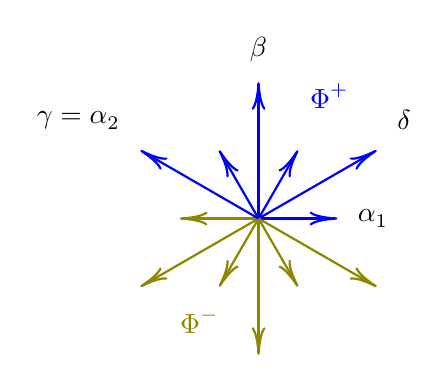
\begin{tikzpicture}[thick, scale=1]
\foreach\ang in {0,60,120}{
  \draw[blue,-{>[length=10,width=5]}] (0,0) -- ++(\ang:1);
  \draw[blue,-{>[length=10,width=5]}] (0,0) -- ++(\ang+30:{sqrt(3)});
  \draw[olive,-{>[length=10,width=5]}] (0,0) -- ++(\ang+180:1);
  \draw[olive,-{>[length=10,width=5]}] (0,0) -- ++(\ang+180+30:{sqrt(3)});
}
\path (0,0) ++(0:1) node [label=right:$\alpha_1$] {};
\path (0,0) ++(150:{sqrt(3)}) node [label=above left:{$\gamma=\alpha_2$}] {};
\path (0,0) ++(90:{sqrt(3)}) node [label=above:$\beta$] {};
\path (0,0) ++(30:{sqrt(3)}) node [label=above right:$\delta$] {};
\node[blue] at (60:1.8) {$\Phi^+$};
\node[olive] at (180+60:1.5) {$\Phi^-$};
\end{tikzpicture}
\end{center}

Пусть теперь $\Phi_i\ne\mathrm{G}_2$. Условие $k\widetilde\beta_i-l\gamma\nprec 0\;\forall k,l\in\N$ выполняется автоматически, если угол между $\gamma$ и $\delta$ составляет $\frac{2\pi}{3}$. Если же угол $\frac{\pi}{2}$, то обеспечить выполнения этого условия можно заменой местами $\gamma$ и $\delta$, чтобы $\delta-\gamma>0$.

\begin{center}
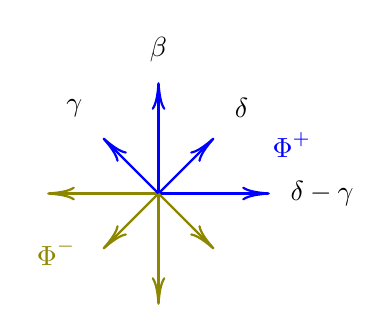
\begin{tikzpicture}[thick, scale=1]
\foreach\ang in {0,90}{
  \draw[blue,-{>[length=10,width=5]}] (0,0) -- ++(\ang:{sqrt(2)});
  \draw[blue,-{>[length=10,width=5]}] (0,0) -- ++(\ang+45:1);
  \draw[olive,-{>[length=10,width=5]}] (0,0) -- ++(\ang+180:{sqrt(2)});
  \draw[olive,-{>[length=10,width=5]}] (0,0) -- ++(\ang+180+45:1);
}
\path (0,0) ++(0:{sqrt(2)}) node [label=right:$\delta-\gamma$] {};
\path (0,0) ++(90+45:1) node [label=above left:{$\gamma$}] {};
\path (0,0) ++(90:{sqrt(2)}) node [label=above:$\beta$] {};
\path (0,0) ++(45:1) node [label=above right:$\delta$] {};
\node[blue] at (20:1.8) {$\Phi^+$};
\node[olive] at (180+30:1.5) {$\Phi^-$};
\end{tikzpicture}
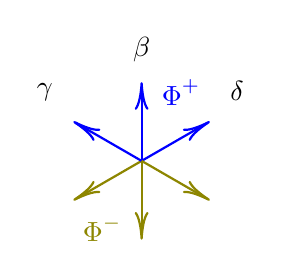
\begin{tikzpicture}[thick, scale=1]
\foreach\ang in {0,60,120}{
  \draw[blue,-{>[length=10,width=5]}] (0,0) -- ++(\ang+30:1);
  \draw[olive,-{>[length=10,width=5]}] (0,0) -- ++(\ang+180+30:1);
}
\path (0,0) ++(150:1) node [label=above left:{$\gamma$}] {};
\path (0,0) ++(90:1) node [label=above:$\beta$] {};
\path (0,0) ++(30:1) node [label=above right:$\delta$] {};
\node[blue] at (60:1) {$\Phi^+$};
\node[olive] at (180+60:1) {$\Phi^-$};
\end{tikzpicture}
\end{center}

В случае, когда $\langle\sigma-\widetilde\beta_i,\widetilde\beta_i\rangle=0$, обеспечить выполнения условия $\langle\sigma,\delta-\gamma\rangle>0$ можно следующим образом. Выберем корень $\delta$, не ортогональный ни $\widetilde\beta_i$, ни $\sigma-\widetilde\beta_i$ (это можно сделать, так как $\Phi$ неприводима и в $\Phi$ есть корень, не ортогональный $\sigma-\widetilde\beta_i$). Не умаляя общности можно считать, что $\langle\delta,\widetilde\beta_i\rangle>0$ и $\langle\delta,\sigma-\widetilde\beta_i\rangle>0$. Тогда $\langle\delta,\widetilde\beta_i\rangle=\frac{1}{2}\langle\widetilde\beta_i,\widetilde\beta_i\rangle$ и $\gamma\coloneqq\widetilde\beta_i-\delta$. При этом
$\langle\sigma,\delta-\gamma\rangle =
\langle\sigma,2\delta-\widetilde\beta_i\rangle =
2\langle\sigma,\delta\rangle-\langle\sigma,\widetilde\beta_i\rangle = 
2\langle\sigma,\delta\rangle-\langle\widetilde\beta_i,\widetilde\beta_i\rangle =
2\langle\delta,\sigma\rangle-2\langle\delta,\widetilde\beta_i\rangle =
2\langle\delta,\sigma-\widetilde\beta_i\rangle > 0$.
Условие $k\widetilde\beta_i-l\gamma\nprec 0\;\forall k,l\in\N$ при этом будет выполнено, так как  $\delta-\gamma$ не может быть отрицательным корнем (если это корень, то положительный).
\end{proof}

\begin{lm}\label{highestweightvariants}
Пусть $\gamma$ и $\delta$ выбраны в соответствии с предыдущей леммой. Тогда
\begin{itemize}[label={\LARGE\raisebox{-0.4ex}{\textbullet}\;},leftmargin=2\parindent]
\item если угол между $\gamma$ и $\delta$ составляет $\frac{2\pi}{3}$, то выполняется хотя бы одно из следующих четырёх условий:
\begin{enumerate}
\item $ \sigma - \gamma \notin \Sigma$
\item $ \sigma - \delta \notin \Sigma$
\item $ \sigma - 2\gamma \in \Sigma$
\item $ \sigma - 2\delta \in \Sigma$
\end{enumerate}
\item если угол между $\gamma$ и $\delta$ составляет $\frac{\pi}{2}$, то выполняется хотя бы одно из следующих четырёх условий:
\begin{enumerate}
\item $ \sigma - 2\gamma \notin \Sigma$
\item $ \sigma - 2\delta \notin \Sigma$
\item $ \sigma - 3\gamma \in \Sigma$
\item $ \sigma - 3\delta \in \Sigma$
\end{enumerate}
\end{itemize}
\end{lm}
\pagebreak

\begin{proof} Докажем, что все четыре условия не могут одновременно нарушаться.
Так как множество весов инвариантно относительно отражений из группы Вейля, то
$$ \sigma - \frac{2 \langle \sigma,\gamma\rangle}{\langle \gamma , \gamma \rangle}\gamma \;\in\; \Sigma $$
$$ \sigma - \frac{2 \langle \sigma,\delta\rangle}{\langle \delta , \delta \rangle}\delta \;\in\; \Sigma \; , $$
но так как $\sigma$ при этом является старшим весом, то
$$ \sigma - \frac{2 \langle \sigma,\gamma\rangle}{\langle \gamma , \gamma \rangle}\gamma-\gamma \;\notin\; \Sigma $$
$$ \sigma - \frac{2 \langle \sigma,\delta\rangle}{\langle \delta , \delta \rangle}\delta-\delta \;\notin\; \Sigma \; . $$

Следовательно, как в случае угла $\frac{2\pi}{3}$ между $\gamma$ и $\delta$ так и в случае угла $\frac{\pi}{2}$, все четыре условия могут одновременно нарушаться, только если $\langle\sigma,\gamma\rangle=\langle\widetilde\beta_i,\gamma\rangle$
и одновременно $\langle\sigma,\delta\rangle=\langle\widetilde\beta_i,\delta\rangle$. Но это значит, что $\langle\sigma-\widetilde\beta_i,\widetilde\beta_i\rangle=0$,
а следовательно по условию предыдущей леммы $\langle\sigma,\delta-\gamma\rangle > 0$, что невозможно, так как $\langle\sigma,\delta-\gamma\rangle = \langle\widetilde\beta_i,\delta-\gamma\rangle = 0$.
\end{proof}

\pagebreak
\section{Основной результат}

Теперь, можно перейти к описанию подгрупп в $P=G\rightthreetimes U$, нормализуемых элементарной группой $E\le G$.

\begin{thm}\label{subgroupprojectionmain}
  Пусть $G = G(\Phi, R)$ --- редуктивная групповая схема Шевалле-Демазюра
  с системой корней $\Phi = \Phi_1 + \ldots + \Phi_n$, где каждая $\Phi_i$ --- неприводимая система корней ранга не менее~$2$. $U$ --- неприводимое над замкнутым полем представление $G$ с таким старшим весом $\widetilde\sigma$, что ни для какой неприводимой компоненты $\Phi_i$ с максимальным весом $\widetilde\beta_i$ разность~${\widetilde\sigma-\widetilde\beta_i}$~не оказывается ортогональна всей $\Phi_i$. В коммутативном кольце $R$ предполагается обратимость всех структурных констант группы $G$, а также в модуле $U$ над кольцом $R$ предполагается выполнение свойства~\refb{returnfromhighest}.
    
  Пусть в параболически-сходной группе $P=G\rightthreetimes U$ имеется подгруппа $H$, нормализуемая группой $E$, то есть $[H,E] \le H$. Тогда образ $H$ при проекции $G \rightthreetimes U \rightarrow G$, обозначаемый как $H_G$, будет обладать следующим свойством: $[H_G,E]\le H$.
\end{thm}
\begin{proof} \quad
$H$ нормализуется $E$, следовательно $H_G$ также нормализуется $E$.
\linebreak
По лемме \refb{directproduct} выполняется $[H_G,E] = \prod_{i=1}^n E(\Phi_i,R,I_i)$ при некотором выборе идеалов $I_i$. Требуется доказать, что $[H_G,E] \le H$, то есть в прямом произведении $\prod_{i=1}^n E(\Phi_i,R,I_i)$ каждый множитель $E(\Phi_i,R,I_i)$  лежит в $H$.

Но по лемме \refb{maximalgenerates} одновременно \vspace{0.8ex} $E(\Phi_i,R,I_i) = X_{\widetilde\beta_i}(I_i)^{E(\Phi_i,R)}$.
Поэтому достаточно доказать, что $X_{\widetilde\beta_i}(I_i)^{E(\Phi_i,R)} \le H$, то есть что
$x_{\widetilde{\beta_i}}(\xi) \in H \ \forall \xi \in I_i$.\vspace{0.8ex}

По построению известно, что $x_{\widetilde\beta_i}(\xi) \in [H_G,E] \le H_G$.
Обозначим за $h$ некоторый прообраз $x_{\widetilde\beta_i}(\xi)$ при проекции $G \rightthreetimes U \rightarrow G$.

\begin{equation*}
\tikzset{
  Subgroup/.style={
    draw=none,
    every to/.append style={
      edge node={node [sloped, allow upside down, auto=false]{$\le$}}}},
  Equals/.style={
    draw=none,
    every to/.append style={
      edge node={node [sloped, allow upside down, auto=false]{$=$}}}},
  Included/.style={
    draw=none,
    every to/.append style={
      edge node={node [sloped, allow upside down, auto=false]{$\in$}}}}
}
\begin{tikzcd}
G \rightthreetimes U \arrow{r}{} & G \\
H \arrow[Subgroup]{u} \arrow{r}{} & H_G \arrow[Subgroup]{u} \\
h \arrow[Included]{u} \arrow[maps to]{r}{} & x_{\widetilde\beta_i}(\xi) \arrow[Included]{u} \\
x_{\widetilde\beta_i}(\xi)\,u \arrow[Equals]{u} \arrow[maps to]{r}{} & x_{\widetilde\beta_i}(\xi) \arrow[Equals]{u} \\
\end{tikzcd}
\end{equation*}


Требуется доказать, что $h$ можно выбрать таким образом, что $u=1$.

\pagebreak

Разложим $u$ по весовым подпространствам:
\begin{equation}\label{weightdecompmain}
u = \prod_{\sigma \in \Sigma} u_\sigma
\end{equation}

Докажем, что все множители, составляющие $u$, принадлежат $H$. Будем доказывать это индукцией по множеству весов, участвующих в произведении.

Пусть $\sigma$ --- минимальный вес из присутствующих в произведении.

Предположим сначала, что $u \notin U_{\widetilde\sigma}$, то есть $u$ не является вектором максимального веса. Докажем переход индукции по аналогии с леммой \refb{weightprojections}.

Для некоторого положительного корня $\alpha_1 \in \Phi$ (не обязательно из $\Phi_i$) вычислим
\begin{multline*}
[x_{\alpha_1}(1), h] = [x_{\alpha_1}(1), x_{\widetilde\beta_i}(\xi)u] =
[x_{\alpha_1}(1), x_{\widetilde\beta_i}(\xi)] \cdot {}^{x_{\widetilde\beta_i}(\xi)}[x_{\alpha_1}(1),u] =\\=
{}^{x_{\widetilde\beta_i}(\xi)}[x_{\alpha_1}(1),u] \; \in \; U \cap H \; .
\end{multline*}

Рассмотрим цепочку положительных корней $\alpha_1,\alpha_2 \ldots \alpha_k$, начинающуюся с $\alpha_1$, такую что $\alpha_1+\alpha_2+\ldots+\alpha_k=\widetilde\sigma-\sigma$. 

Последовательное коммутирование $u_\sigma$ с корневыми элементами этой цепочки приводит к такому же результату, как действие оператора $\varepsilon_{\alpha_k}(1)\ldots\varepsilon_{\alpha_2}(1)\,\varepsilon_{\alpha_1}(1)$:
$$ [x_{\alpha_k}(1),[\ldots[x_{\alpha_2}(1),[x_{\alpha_1}(1),u_\sigma]]\ldots]] =
\big(\varepsilon_{\alpha_k}(1)\ldots\varepsilon_{\alpha_2}(1)\varepsilon_{\alpha_1}(1)\big)(u_\sigma) \;.$$
При этом к тому же результату приводит и аналогичное коммутирование $u$:
$$ [x_{\alpha_k}(1),[\ldots[x_{\alpha_2}(1),[x_{\alpha_1}(1),u]]\ldots]] =
\big(\varepsilon_{\alpha_k}(1)\ldots\varepsilon_{\alpha_2}(1)\varepsilon_{\alpha_1}(1)\big)(u_\sigma) \;,$$
и тот же результат получается при аналогичном коммутировании $h$:
\begin{multline*}
[x_{\alpha_k}(1),[\ldots[x_{\alpha_2}(1),[x_{\alpha_1}(1),h]]\ldots]] =\\=
[x_{\alpha_k}(1),[\ldots[x_{\alpha_2}(1),{}^{x_{\widetilde\beta_i}(\xi)}[x_{\alpha_1}(1),u]]\ldots]] =\\=
[x_{\alpha_k}(1),[\ldots{}^{x_{\widetilde\beta_i}(\xi)}[x_{\alpha_2}(1),[x_{\alpha_1}(1),u]]\ldots]] =\\=
{}^{x_{\widetilde\beta_i}(\xi)}[x_{\alpha_k}(1),[\ldots[x_{\alpha_2}(1),[x_{\alpha_1}(1),u]]\ldots]] =\\=
\big(\varepsilon_{\alpha_k}(1)\ldots\varepsilon_{\alpha_2}(1)\varepsilon_{\alpha_1}(1)\big)(u_\sigma) \;,
\end{multline*}

Из этого можно заключить, что $\big(\varepsilon_{\alpha_k}(1)\ldots\varepsilon_{\alpha_2}(1)\varepsilon_{\alpha_1}(1)\big)(u_\sigma) \; \in \; H$ для всех цепочек положительных корней $\alpha_1\ldots\alpha_k$, а следовательно, по свойству \refb{returnfromhighest} $u_\sigma \in H$. Таким образом, доказан переход индукции, то есть число множителей в разложении (\ref{weightdecompmain}) можно уменьшить, выбрав другой прообраз $h$.

Докажем теперь базу индукции, то есть случай, когда $u \in  U_{\widetilde\sigma}$.
Представим $\beta\coloneqq\widetilde\beta_i$ в виде суммы $\gamma+\delta$ в соответствии с леммой~\refb{maxrootsum}.

\pagebreak


Предварительно выделим и отдельно рассмотрим случай, когда $\widetilde\sigma-\delta+\gamma \in \Sigma$. В этом случае
\begin{multline*}
[x_{\gamma-\delta}(1),h] = [x_{\gamma-\delta}(1),x_\beta(\xi)u] = [x_{\gamma-\delta}(1),x_\beta(\xi)] \cdot {}^{x_\beta(\xi)}[x_{\gamma-\delta}(1),u] =\\=
{}^{x_\beta(\xi)}[x_{\gamma-\delta}(1),u] \;\in\; U\cap H \;.
\end{multline*}
Очевидно, $\widetilde\sigma + \N(\gamma-\delta)+\N\beta \notin \Sigma$, поэтому
$h_{-\gamma} = [x_{-\gamma}(1),u]$. Дальнейшее коммутирование с $x_{\gamma-\delta}(1)$ приводит к элементу $w\coloneqq\varepsilon_{\gamma-\delta}(1)^k(u)$, $k=2\frac{\langle\sigma,\delta-\gamma\rangle}{\langle\delta-\gamma,\delta-\gamma\rangle}$, лежащему в подпространстве экстремального веса $\sigma-2\frac{\langle\sigma,\delta-\gamma\rangle}{\langle\delta-\gamma,\delta-\gamma\rangle}(\delta-\gamma)$. Так как $w\in H$, то по лемме \refb{extremalweightisomorphism} также $u \in H$.

Пусть теперь $\widetilde\sigma-\delta+\gamma \notin \Sigma$. В этом случае $\N\beta-\N\delta$, так же как и $\N\beta-\N\gamma$, будут неотрицательны.

Обозначим
\begin{multline*}
h_{-\gamma} \coloneqq [x_{-\gamma}(1),h] = [x_{-\gamma}(1),x_\beta(\xi) u] = [x_{-\gamma}(1),x_\beta(\xi)] \cdot {}^{x_\beta(\xi)}[x_{-\gamma}(1),u] = \\ =
x_{\beta-\gamma}(N_{-\gamma,\beta,1,1} \,\xi) \, x_{\beta-2\gamma}(\ldots) \, \varepsilon_{-\gamma}(u) \, u_1 \; ,
\end{multline*}
где $u_1$ раскладывается по подпространствам $U_\sigma$ с $\sigma \in \widetilde\sigma-\gamma - \N \, \gamma$ (абстрактные веса $\{\widetilde\sigma-\N\,\gamma+\N\,\beta\}$ не могут являться весами представления, так как среди $\{\N\,\beta-\N\,\gamma\}$ нет отрицательных абстрактных весов).

\begin{center}
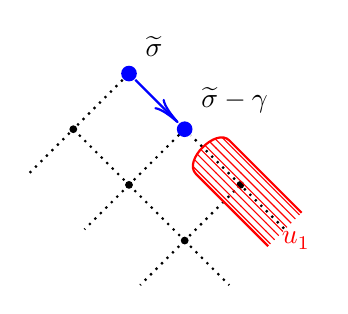
\begin{tikzpicture}[thick, scale=1]
\newcommand{\point}[1]{node (#1) [circle,inner sep=1,fill] {}}
\draw[dotted] (0,0) node (sigma) [circle,inner sep=2,fill=blue,label=above right:{$\widetilde\sigma$}] {} ++(-45:1) node (sigmaminusgamma) [circle,inner sep=2,fill=blue,label=above right:{$\widetilde\sigma-\gamma$}] {} -- ++(-90-45:1) \point{} -- ++(90+45:1) \point{} -- +(-90-45:0.8) ++(-45:1) -- +(-90-45:0.8) ++(0:0) -- ++(-45:1) \point{} -- ++(45:1) \point{} -- +(-45:0.8) ++(-90-45:1) -- +(-45:0.8) ++(0:0) -- +(-90-45:0.8) ++(45:1) -- (sigmaminusgamma) (sigma) -- +(-90-45:1);
\draw[blue,-{>[length=10,width=5]}] (sigma) -- (sigmaminusgamma);
\draw[red,pattern=north west lines, pattern color=red] (-45:2.8) ++(45:0.3) -- ++(90+45:1.3) to[bend right=90] ++(-90-45:0.6) -- ++(-45:1.3) ++(45:0.3);
\node[red] at (-45:3.0) {$u_1$};
\end{tikzpicture}
\end{center}

\begin{multline*}
h_{-2\gamma} \coloneqq [x_{-\gamma}(1),h_{-\gamma}] = \\ =
[x_{-\gamma}(1), x_{\beta-\gamma}(N_{-\gamma,\beta,1,1} \,\xi) \, x_{\beta-2\gamma}(\ldots) \, \varepsilon_{-\gamma}(u) \, u_1] = \\ =
[x_{-\gamma}(1), x_{\beta-\gamma}(N_{-\gamma,\beta,1,1} \,\xi) \, x_{\beta-2\gamma}(\ldots)] \cdot \\ \cdot {}^{x_{\beta-\gamma}(N_{-\gamma,\beta,1,1} \,\xi) \, x_{\beta-2\gamma}(\ldots)} [x_{-\gamma}(1), \varepsilon_{-\gamma}(u) \, u_1] = \\ =
x_{\beta-2\gamma}(N_{-\gamma,\beta,1,1} N_{-\gamma,\beta-\gamma,1,1} \, \xi) \; \varepsilon^2_{-\gamma}(u) \, u_2 \; ,
\end{multline*}
где $u_2$ раскладывается по подпространствам $U_\sigma$ с $\sigma \in \widetilde\sigma-2\gamma - \N \, \gamma$.

\begin{center}
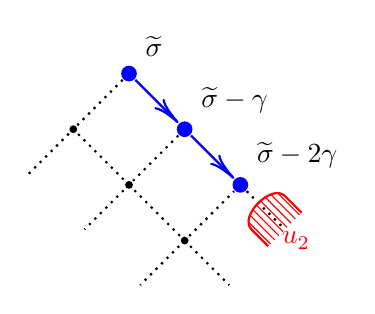
\begin{tikzpicture}[thick, scale=1]
\newcommand{\point}[1]{node (#1) [circle,inner sep=1,fill] {}}
\draw[dotted] (0,0) node (sigma) [circle,inner sep=2,fill=blue,label=above right:{$\widetilde\sigma$}] {} ++(-45:1) node (sigmaminusgamma) [circle,inner sep=2,fill=blue,label=above right:{$\widetilde\sigma-\gamma$}] {} ++(-45:1) node (sigmaminus2gamma) [circle,inner sep=2,fill=blue,label=above right:{$\widetilde\sigma-2\gamma$}] {} (sigmaminusgamma) -- ++(-90-45:1) \point{} -- ++(90+45:1) \point{} -- +(-90-45:0.8) ++(-45:1) -- +(-90-45:0.8) ++(0:0) -- ++(-45:1) \point{} -- (sigmaminus2gamma) -- +(-45:0.8) ++(-90-45:1) -- +(-45:0.8) ++(0:0) -- +(-90-45:0.8) (sigma) -- +(-90-45:1);
\draw[blue,-{>[length=10,width=5]}] (sigma) -- (sigmaminusgamma);
\draw[blue,-{>[length=10,width=5]}] (sigmaminusgamma) -- (sigmaminus2gamma);
\draw[red,pattern=north west lines, pattern color=red] (-45:2.8) ++(45:0.3) -- ++(90+45:0.3) to[bend right=90] ++(-90-45:0.6) -- ++(-45:0.3) ++(45:0.3);
\node[red] at (-45:3.0) {$u_2$};
\end{tikzpicture}
\end{center}

Аналогично вводятся $h_{-\delta}$ и $h_{-2\delta}$, а также $h_{-3\gamma}$ и $h_{-3\delta}$.
\begin{multline*}
h_{-3\gamma} \coloneqq [x_{-\gamma}(1),h_{-2\gamma}] = \\ =
[x_{-\gamma}(1), x_{\beta-2\gamma}(N_{-\gamma,\beta,1,1} N_{-\gamma,\beta-\gamma,1,1} \, \xi) \; \varepsilon^2_{-\gamma}(u) \, u_2] = \\ =
{}^{x_{\beta-2\gamma}(N_{-\gamma,\beta,1,1} N_{-\gamma,\beta-\gamma,1,1} \, \xi)}[x_{-\gamma}(1),\varepsilon^2_{-\gamma}(u) \, u_2] =
\varepsilon^3_{-\gamma}(u) \, u_3
 \; ,
\end{multline*}
где $u_3$ раскладывается по подпространствам $U_\sigma$ с $\sigma \in \widetilde\sigma-3\gamma - \N \, \gamma$.

Рассмотрим варианты в соответствии с леммой \refb{highestweightvariants}.
\begin{itemize}[label={\LARGE\raisebox{-0.4ex}{\textbullet}\;},leftmargin=2\parindent]
\item Если угол между $\gamma$ и $\delta$ составляет $\frac{2\pi}{3}$:
\begin{enumerate}
\item $ \sigma - \gamma \notin \Sigma$, тогда $h_{-\gamma}=x_{\beta-\gamma}(N_{-\gamma,\beta,1,1} \,\xi)\in E\cap H$ и $x_\beta(\xi)\in H$
\item $ \sigma - \delta \notin \Sigma$, тогда $h_{-\delta}=x_{\beta-\delta}(N_{-\delta,\beta,1,1} \,\xi)\in E\cap H$ и $x_\beta(\xi)\in H$
\item $ \sigma - 2\gamma \in \Sigma$, тогда $h_{-2\gamma}=\varepsilon_{-\gamma}^2(u)\in U\cap H$ и по лемме \refb{extremalweightisomorphism} $u\in H$
\item $ \sigma - 2\delta \in \Sigma$, тогда $h_{-2\delta}=\varepsilon_{-\delta}^2(u)\in U\cap H$ и по лемме \refb{extremalweightisomorphism} $u\in H$
\end{enumerate}
\item Если угол между $\gamma$ и $\delta$ составляет $\frac{\pi}{2}$:
\begin{enumerate}
\item $ \sigma - 2\gamma \notin \Sigma$, тогда $h_{-2\gamma}=x_{\beta-2\gamma}(N_{-\gamma,\beta,1,1}N_{-\gamma,\beta-\gamma,1,1} \,\xi)\in E\cap H$ и $x_\beta(\xi)\in H$
\item $ \sigma - 2\delta \notin \Sigma$, тогда $h_{-2\delta}=x_{\beta-2\delta}(N_{-\delta,\beta,1,1}N_{-\delta,\beta-\delta,1,1} \,\xi)\in E\cap H$ и $x_\beta(\xi)\in H$
\item $ \sigma - 3\gamma \in \Sigma$, тогда $h_{-3\gamma}=\varepsilon_{-\gamma}^3(u)\in U\cap H$ и по лемме \refb{extremalweightisomorphism} $u\in H$
\item $ \sigma - 3\delta \in \Sigma$, тогда $h_{-3\delta}=\varepsilon_{-\delta}^3(u)\in U\cap H$ и по лемме \refb{extremalweightisomorphism} $u\in H$
\end{enumerate}
\end{itemize}

Таким образом мы доказали, что максимальные корневые элементы $x_{\widetilde\beta_i}(\xi)$, лежащие в~$[H_G,E]$, также лежат и в $H$, что и требовалось доказать.

\end{proof}

Теперь, когда мы увидели, что в $G$ содержится достаточно большая подгруппа, коммутант которой с $E$ лежит в $H$, структуру подгруппы $H$ описать достаточно легко. Сначала рассмотрим случай, когда $H$ целиком содержится в унипотентном радикале $U$, а затем докажем общий случай.

\newpage
\begin{lm}\label{unipotenttransitivity}
  Любая подгруппа $H \le U$, нормализуемая $G$, имеет вид $U_I$, где $I$ --- идеал кольца.
\end{lm}
\begin{proof}
Данное утверждение непосредственно вытекает из леммы \refb{unipotentsubgroups} и является её переформулировкой с использованием мультипликативной записи.
\end{proof}
\begin{thm}
В условиях предыдущей теоремы подгруппа $H\le G \rightthreetimes U$ может быть представлена в виде $H = H_G \rightthreetimes H_U$, где $[H_G,E] = \prod_{i=1}^n E(\Phi_i, R, I_i)$, а $H_U=U_I$ --- подмодуль $U$, заданный некоторым идеалом кольца.
\end{thm}
\begin{proof}
Достаточно доказать, что $H_G \le H$, оставшаяся часть следует из леммы~\refb{unipotenttransitivity}. \#

Разложим элемент $h \in H$ в произведение $h = z u$, где $z \in H_G$, $u \in U$. Докажем, что $z$ и $u$ также лежат в $H$.

Прокоммутируем $h$ с некоторым $g$ из $E$:
$$ [g, h] = [g,zu] = [g,z] \cdot {}^z[g,u] $$

По теореме \refb{subgroupprojectionmain} $[g,z]\in H$, следовательно, ${}^z[g,u]$ так же лежит в $H$. Но
$ {}^z[g,u] = {}^{zu}[u^{-1},g] $, следовательно, $[u^{-1},g] \in H$. Выбирая в качестве $g$ корневые элементы $x_\alpha(1)$ с корнями из начала цепочек, возникающих в формулировке свойства \refb{returnfromhighest}, получим, что $u$ также лежит~в~$H$.
\end{proof}

Таким образом, оказывается, что если проекция старшего веса $\sigma$ на линейную оболочку каждой неприводимой компоненты $\Phi_i$ не совпадает с максимальным корнем этой компоненты, то любая подгруппа $H \le P$, нормализуемая $E$, распадается в полупрямое произведение двух подгрупп, также нормализуемых $E$, одна из которых целиком лежит в редуктивной группе $G$, а другая унипонентна.

\pagebreak
\section{Случай присоединённого представления}

Описанный выше результат о виде подгрупп, нормализуемых $E$, получен при выполнении предположений теоремы \refb{subgroupprojectionmain}. Среди этих условий выделяется условие о том, что все $\widetilde\sigma-\widetilde\beta_i$ не ортогональны соответствующим $\Phi_i$. Это требование вытекает из леммы \refb{maxrootsum} и отделяет случай, когда для некоторого $\Phi_i$ оказывается $\widetilde\sigma-\widetilde\beta_i$ ортогонально $\Phi_i$. Этот случай является существенным исключением, и для него выполняется более слабый результат.

\begin{thm}
Пусть выполняются условия теоремы \refb{subgroupprojectionmain} за исключением требования $\widetilde\sigma-\widetilde\beta_i \not\perp \Phi_i \; \forall i$. А именно, пусть для некоторого $i$ выполнено $\widetilde\sigma-\widetilde\beta_i \perp \Phi_i$.

Тогда если $x_{\widetilde\beta_i}(\xi) \in H_G$, то $x_{\widetilde\beta_i}(\xi^2) \in H$.
\end{thm}
\begin{proof}
Как известно, системы корней $A_n$ при $n\ge 2$, $B_n$ и $C_n$ при $n\ge 3$, $D_n$ при $n\ge 3$, а также $E_6$, $E_7$, $E_8$, $F_4$ и $G_2$ содержат в себе систему корней $A_2$, проходящую через максимальный корень. Докажем теорему сначала для этого случая. Пусть $\gamma+\delta=\widetilde\beta_i$, и угол между $\gamma$ и $\delta$ составляет $\frac{2\pi}{3}$.

Тогда
\begin{equation*}
\begin{split}
x_{\gamma+\delta}(\xi^2) = & \\
& \quad [x_\delta(-1),[x_{\gamma+\delta}(1), \\
& \quad\qquad \phantom{{}\cdot{}} [x_{-\delta}(1),[x_{-\gamma-\delta}(1),x_{\gamma+\delta}(\xi) \cdot u]] \cdot {} \\
& \quad\qquad \cdot [x_{-\delta}(-2\xi),x_{\gamma+\delta}(\xi) \cdot u] \cdot {} \\
& \quad\qquad \cdot [x_{-\gamma-\delta}(-2\xi-1),[x_{-\delta}(1),x_{\gamma+\delta}(\xi) \cdot u]] \\
& \quad ]] \in H
\end{split}
\end{equation*}

Если же система корней $\Phi_i$ не содержит в себе $A_2$, проходящую через максимальный корень, то $\Phi_i \cong C_2$. В этом случае пусть $\gamma+\delta=\widetilde\beta_i$, и угол между $\gamma$ и $\delta$ составляет $\frac{\pi}{2}$.
Тогда
\begin{equation*}
\begin{split}
x_{\gamma+\delta}(4\xi^2) = & \\
& \quad [x_\delta(1),[x_\delta(1), \\
& \quad\qquad \phantom{{}\cdot{}} [x_\gamma(1),\\
& \quad\qquad\qquad \phantom{{}\cdot{}} [x_{-\delta}(1),[x_{-\gamma-\delta}(1),x_{\gamma+\delta}(\xi ) \cdot u]] \cdot{} \\
& \quad\qquad\qquad {}\cdot [x_{-\delta}(-2 \xi ),x_{\gamma+\delta}(\xi ) \cdot u]\\
& \quad\qquad \phantom{{}\cdot{}} ] \cdot{} \\
& \quad\qquad {}\cdot [x_{-\delta}(2 \xi +1),[x_{-\delta}(1),x_{\gamma+\delta}(\xi ) \cdot u]] \\
& \quad ]] \in H
\end{split}
\end{equation*}
\end{proof}

\pagebreak
\section{Обобщение на случай неабелева унипотентного радикала}

Группы, рассматриваемые в предыдущих разделах, являются нередуктивными линейными алгебраическими группами с абелевым унипотентным радикалом.

Перейдём теперь к рассмотрению групп, получающихся подобным же образом из представлений, но в которых унипонетный радикал будет уже не абелев, в класса нильпотентности 2, то есть коммутант унипотентного радикала будет абелевым.

\begin{framed}
\begin{definition}
Пусть $U$ --- $G$-модуль, являющийся алгеброй над $R$ с умножением, которое согласовано с действием $G$:
$$\circledast : U \times U \to U$$
$$ {}^g u \circledast {}^g v = {}^g (u \circledast v) .$$

При этом, обозначив $V:=U\circledast U$, будем предполагать, что $U$ раскладывается в прямую сумму $U = U/V \oplus V$.

Тогда можно рассмотреть группу $P$, являющуюся расширением $G$ с помощью $U$, элементами которой будут пары $(g,u)$, $g \in G$, $u \in U$ со следующим умножением:
$$
(g,u)\cdot (g',u') = (g g', {}^{g'^{-1}} u + u' + {}^{g'^{-1}} u \circledast u')
$$

Назовём такую группу \textit{\textbf{параболически-сходной группой с унипотентным радикалом класса нильпотентности 2}}.
\end{definition}
\end{framed}

\begin{example}
Если $V=0$, то есть $u \circledast u'$ всегда тривиально, то эта конструкция представляет собой полупрямое произведение группы $G$ и аддитивной группы модуля $U$.
\end{example}

Если же $u \circledast u'$ нетривиально, то $P$ тоже является полупрямым произведением группы $G$, но уже с группой, состоящей из элементов из $U$ с умножением
$
(u,u') \mapsto u + u' + u \circledast u'
$.

\begin{example}
Частным случаем предыдущего примера является пример, когда группа $G$ является прямым произведением групп $G_1,\ldots ,G_n$, а модуль $U$ раскладывается в прямую сумму $U_1 \oplus \ldots \oplus U_{n-1}$ со следующими действиями групп на них:
\begin{equation*}
\begin{array}{lcccr}
G_1 & \lacts & U_1 & \racts & G_2 \\
\hdotsfor{5}\\
G_{n-1} & \lacts & U_{n-1} & \racts & G_n
\end{array}
\end{equation*}

Тогда действие $G$ на $U$ конструируется из левых и правых действий $G_1\ldots G_n$ следующим образом:
\begin{equation*}
(g_1,\ldots , g_n) : u_i \mapsto g_i u_i g_{i+1}^{-1}
\end{equation*}


В результате $P = G \rightthreetimes U$ можно записать как факторгруппу группы матриц вида
\begin{equation*}
\begin{pmatrix}
g_1 & g_1 u_1 &     &     & \bigzero{*}{-2} \\
    & g_2 & g_2 u_2 & &  \\
    &    &\ddots&\ddots&    \\
    &     &     &g_{n-1}& g_{n-1} u_{n-1} \\
\bigzero{$0$}{3}& &     &     & g_n \\
\end{pmatrix}
\end{equation*}

по подгруппе вида
\begin{equation*}
\begin{pmatrix}
1 & 0 &      &      & \bigzero{*}{-2} \\
  & 1 & 0    &      &   \\
  &   &\ddots&\ddots&   \\
  &   &      &1     & 0 \\
\bigzero{$0$}{3}&&&   & 1 \\
\end{pmatrix}
\end{equation*}
\end{example}

\begin{example}
Обобщая предыдущий пример на случай $V\neq0$, можно рассмотреть факторгруппу матриц вида
\begin{equation*}
\resizebox{.9\hsize}{!}{$
\left.
\begin{pmatrix}
g_1 & g_1 u_1 & g_1 v_1 &      & &  & \bigzero{*}{-1}        \\
    & g_2     & g_2 u_2 & \ddots &    &  &  \\
    &         & g_3     & \ddots  & \ddots &  &    \\
    &         &         & \ddots  & \ddots & \ddots  &    \\
    &      &  & & g_{n-2}     & g_{n-2} u_{n-2} & g_{n-2} v_{n-2} \\
    &      &  & &         & g_{n-1}     & g_{n-1} u_{n-1} \\
\bigzero{$0$}{3} & &  &  &    &         & g_n     \\
\end{pmatrix}
\right/
\begin{pmatrix}
  1 &       0 & 0       &        & \bigzero{*}{-1}  \\
    & \ddots  & \ddots  & \ddots &                  \\
    &         & 1       & 0      & 0                \\
    &         &         & 1      & 0                \\
\bigzero{$0$}{3} & &      &        & 1                \\ 
\end{pmatrix}
$},
\end{equation*}

где
\begin{equation*}
\resizebox{.9\hsize}{!}{$
\begin{array}{lcccr}
G_1 & \lacts & U_1 & \racts & G_2 \\
\hdotsfor{5}\\
G_{n-1} & \lacts & U_{n-1} & \racts & G_n\\
\vspace{3ex}\\
G_1 & \lacts & V_1 & \racts & G_3 \\
\hdotsfor{5}\\
G_{n-2} & \lacts & V_{n-2} & \racts & G_n
\end{array}
$
\qquad
$
\begin{array}{lcccr}
\circledast & : & U_1 \times U_2 & \to & V_1 \\
\hdotsfor{5}\\
\circledast & : & U_{n-2} \times U_{n-1} & \to & V_{n-2}
\end{array}
$}
\end{equation*}

При этом согласованность операции $\circledast$ с действиями групп означает, что
\begin{multline*}
(g_1 u_1 g_2^{-1}, \ldots, g_{n-1} u_{n-1} g_n^{-1}) \circledast (g_1 u'_1 g_2^{-1}, \ldots, g_{n-1} u'_{n-1} g_n^{-1}) 
= \\ =
(g_1 u_1 g_2^{-1} g_2 u'_2 g_3^{-1}, \ldots) = 
(g_1 u_1 u'_2 {g}_3^{-1}, \ldots, g_{n-2} u_{n-2} u'_{n-1} g_n^{-1}).
\end{multline*}
\end{example}

\begin{example}
Чтобы группа $P$ была похожа на параболические подгруппы, нужно дополнительно потребовать, чтобы $U \circledast V = V \circledast U = 0$, то есть чтобы
$$ \circledast : U/V \times U/V \to V.$$

Тогда результирующая группа будет состоять из троек $(g,u,v)$, $g \in G$, $u \in U/V$, $v \in V$ со следующим умножением:
$$
(g,u,v)\cdot (g',u',v') = (g g', {}^{g'^{-1}} u + u', {}^{g'^{-1}} v + v' + {}^{g'^{-1}} u \circledast u').
$$
\end{example}

\begin{thm}
Пусть $P$ --- параболически-сходная группа над $R$ с унипотентным радикалом класса нильпотентности 2, построенная по представлению $U$ группы $G$ со структурой алгебры~${\circledast}$ на представлении, причём  $U=V \oplus U/V$, где $V:=U\circledast U$.

Тогда если $V$ и $U/V$ --- простые представления группы $G$, для которых с учётом выбора кольца $R$ выполняется свойство \refb{returnfromhighest}, то подгруппы унипотентного радикала, нормализуемые $E$, задаются парой идеалов $I$, $J$, где $I^2 \subset J$.
\end{thm}
\begin{proof}
Пусть $U'\le U$ --- подгруппа, нормализуемая $E$. Так как $P$ допускает факторизацию по $V$, то в $U/V$ будет подгруппа $U'/V$, так же нормализуемая $E$. Аналогично, в $V$ есть подгруппа $U' \cap V$, нормализуемая $E$. А так как $E$-инвариантные подмодули в $U/V$ и в $V$ определяются утверждением \refb{unipotentsubgroups}, то осталось доказать, что $I^2 \subset J$. Но это следует из замкнутости подмодуля относительно~${\circledast}$.
\end{proof}

Если $V$ и $U/V$ --- простые представления, то они раскладываются по весовым пространствам. Следующая лемма говорит о том, что операция~${\circledast}$ согласована с весовым разложением.

\begin{thm}
Если $u,u' \in U/V$ --- векторы весов $\sigma, \sigma'$, то $u \circledast u' \in V$ --- вектор веса $\sigma + \sigma'$.
\end{thm}
\begin{proof}
$$
{}^h(u \circledast u') = {}^h u  \circledast {}^h u' = \sigma(h) u \; \circledast \; \sigma'(h) u' = \sigma(h)\sigma'(h) \enspace u \circledast u'
$$
\end{proof}


Приведённые выше доказательства  и примеры подтвердают корректность и осмымленность предложенного определения параболически-сходных групп с унипотентным радикалом класса нильпотентности 2.
Наличие согласованного с действием $G$ весового разложения позволяет предположить, что для параболически-сходных групп с унипотентным радикалом класса нильпотентности~2 может быть получен результат, аналогичный теореме \refb{subgroupprojectionmain}.

\section{Заключение}

В настоящей работе получено доказательство теоремы о нормальном строении сходных с параболическими линейных алгебраических групп с абелевым унипотентным радикалом.
А именно, установлено, что при соблюдении некоторых условий, касающихся решётки весов, любая подгруппа, нормализуемая элементарной, распадается в полупрямое произведение части, содержащейся в редуктивной подгруппе, и унипотентной части. В исключительном случае, когда проекция старшего веса на одну из неприводимых компонент системы корней совпадает с соответствующим максимальным корнем, вычисления на решётках корней, положенные в основу доказательства, неприменимы, и в этом случае выполняется более слабое условие на подгруппы, нормализуемые элементарной.

Также в работе сформулировано обобщающее понятие сходных с параболическими линейных алгебраических групп с унипотентным радикалом класса нильпотентности не более~2. Описание нормального строения для данного класса групп является предметом дальнейших исследований.
Также представляет интерес возможность дальнейшего обобщения результатов данной работы на аналогичные по строению нередуктивные группы с унипотентным радикалом более высокого класса нильпотентности.

\bibliographystyle{ugost2008ls}
\bibliography{references}

\end{document}

